\documentclass[9pt,lineno]{elife}

%%%%%%%%%%%%%%%%%%%%%%%%%%%%%%%%%%% table
\usepackage{multirow}

%%%%%%%%%%%%%%%%%%%%%%%%%%%%%%%%%% font size %%%%%%%%%%%%%%%%%%%%%%%%
\usepackage{anyfontsize}

%%%%%%%%%%%%%%%%%%%%%%%%%%%%%%%%%% Maths %%%%%%%%%%%%%%%%%%%%%%%%%%%%
\usepackage{amsmath}

%%%%%%%%%%%%%%%%%%%%%%%%%%%%%%%%%% referencing %%%%%%%%%%%%%%%%%%%%%%%%%%%%%%%%%%
%\usepackage{natbib}
\usepackage{hyperref}
\usepackage{xcolor}
\hypersetup{
    colorlinks,
    %linkcolor={red!50!black},
    linkcolor={black},
    citecolor={blue!50!black},
    urlcolor={blue!80!black}
}

%%%%%%%%%%%%%%%%%%%%%%%%%%%%%%%%%% figure and table %%%%%%%%%%%%%%%%%%%%%%%%%%%%%%%%%%
\usepackage{graphicx}
\graphicspath{{./figures/}}
%\graphicspath{{}}
\usepackage[label font=bf,labelformat=simple, position = top]{subfig}
\newdimen\figrasterwd
\figrasterwd\textwidth
\usepackage{wrapfig}
\usepackage{lipsum}

%%%%%%%%%%%%%%%%%%%%%%%%%%%%%%%%%% layout %%%%%%%%%%%%%%%%%%%%%%%%%%%%%%%%%%
\usepackage{setspace}
\linespread{1.5}
\usepackage{authblk}

%\usepackage{fancyhdr}
\providecommand{\keywords}[1]{\textbf{\textit{Key words:}} #1}

%\newcommand\@shorttitle{}
% define \theshorttitle to what is given
%\newcommand\shorttitle[1]{\renewcommand\@shorttitle{#1}}

%%%%%%%%%%%%%%%%%%%%%%%%%%%%%%%%%% todo %%%%%%%%%%%%%%%%%%%%%%%%%%%%%%%%%%
%\usepackage[colorinlistoftodos]{todonotes}
\usepackage[disable]{todonotes}

\newcounter{todocounter}
\newcommand{\todonum}[2][]
{\stepcounter{todocounter}\todo[#1]{\thetodocounter: #2}}

\newcommand{\done}[2][]
{\todo[color=green!40, #1]{#2}}
\newcommand{\donenum}[2][]
{\stepcounter{todocounter}\done[#1]{\thetodocounter: #2}}


\newcommand{\narrative}[2][]
{\todo[color=blue!40, #1]{#2}}
\newcommand{\narrativenum}[2][]
{\stepcounter{todocounter}\narrative[#1]{\thetodocounter: #2}}

\newcommand{\donenarrative}[2][]
{\todo[color=green!40, #1]{#2}}
\newcommand{\donenarrativenum}[2][]
{\stepcounter{todocounter}\narrative[#1]{\thetodocounter: #2}}



\begin{document}

\title{Characterising local epidemiology of {\it P. falciparum} malaria through the structure of mixed infections}
\newcommand\shorttitle{Mixed infections in malaria}
\date{}

\author[?]{(LIST OF NAMES, NEEDS ORDERING)}
\author[1]{Sha Joe Zhu}
\author[1,2,3,4]{Jacob Almagro-Garcia}
\author[1]{Jason Hendry}
\author[2,3]{Richard Pearson}
\author[2,3]{Alistair Miles}
\author[2,3]{Roberto Amato}
\author[?]{Pf3k Consortium}
\author[2,3]{Dominic Kwiatkowski}
\author[1,3]{Gil McVean}

\corr{gil.mcvean@bdi.ox.ac.uk}{GM}

\affil[1]{Big Data Institute, Li Ka Shing Centre for Health Information and Discovery, University of Oxford}
\affil[2]{Wellcome Centre for Human Genetics, University of Oxford}
\affil[3]{Medical Research Council Centre for Genomics and Global Health, University of Oxford}
\affil[4]{Wellcome Trust Sanger Institute}
%\donenum[inline]{updated affiliation}
%}

\maketitle{}

\begin{abstract}
Individuals infected with the {\it Plasmodium falciparum} malaria parasite can carry multiple strains with varying levels of relatedness. Yet how parameters of local epidemiology and the biology of transmission affect the rate and relatedness of such mixed infections remains unclear.  Here, we develop an enhanced method for strain deconvolution from genome sequencing data, which estimates the number of strains, their proportions, identity-by-descent (IBD) profiles and individual haplotypes.  We validate the method through experimental and {\em in silico} simulations and apply it to the Pf3k data set, consisting of 2,344 field samples from 13 countries.  We find that the rate of mixed infection varies from 18\% to 63\% across countries and that 51\% of all mixed infections involve more than two strains.  By modelling the structure of IBD resulting from different infection mechanisms we estimate that 55\% of dual infections contain sibling strains likely to have been co-transmitted from a single mosquito and find evidence of mixed infections propagated over successive infection cycles.  By combining genetic data with epidemiological estimates of prevalence from the Malaria Atlas Project, we find that, at a country level, prevalence correlates with both the rate of mixed infection (Pearson $r = 0.65$, P $= 3.7 \times 10^{-6}$) and the level of IBD ($r = -0.51$, $P = 6.0 \times 10^{-4}$).  We conclude that monitoring spatial and temporal patterns of mixed infection and relatedness between strains will be highly informative in pathogen surveillance and assessing the impact of interventions.
\end{abstract}

\keywords{Malaria, genome, epidemiology, relatedness}


\section{Introduction}


Individuals infected with malaria-causing parasites of the genus {\it Plasmodium} often carry multiple, distinct strains of the same species ~\citep{Bell2006}.  Such mixed infections are likely indicative of intense local exposure rates, being common in regions of Africa with high rates of prevalence~\citep{Howes2016}. However, they have also been documented for {\it P.~vivax} and other malaria-causing parasites~\citep{Mueller2007, Collins2012}, even in regions of much lower prevalence~\citep{Howes2016, Steenkeste2010}.  Mixed infections have been associated with increased disease severity \citep{deRoode2005} and also facilitate the generation of genomic diversity within the parasite, enabling co-transmission to the mosquito vector where sexual recombination occurs \citep{Mzilahowa2007}.  Mixed infections are transient \citep{Bruce2002, Zimmerman2004}, but little is known about the distribution of their duration. Whether the clearance of one or more strains results purely from host immunity~\citep{Borrmann2011} or can be influenced by interactions between the distinct strains~\citep{Enosse2006, Bushman2016}, are also open questions.

Although mixed infections can be studied from genetic barcodes~\citep{Galinsky2015} or single nucleotide polymorphisms (SNPs)~\citep{Jack2016}, genome sequencing provides a more powerful approach for detecting mixed infections~\citep{Chang2017}.  Genetic differences between co-existing strains manifest as polymorphic loci in the sequence of the isolate. The higher resolution of sequencing data allows the use of statistical methods for estimating the number of distinct strains, their relative proportions, and genome sequences~\citep{Zhu2017}.  Although genomic approaches cannot identify individuals infected multiple times by identical strains, and are affected by sequencing errors and problems of incomplete or erroneous reference assemblies, they provide a rich characterisation of within host diversity~\citep{Manske2012}.

Previous research has highlighted that co-existing strains can be highly related~\citep{Nair2014, Trevino2017}.  For example, in {\it P. vivax}, 58\% of mixed infections show long stretches of within host homozygosity~\citep{Pearson2016}. In addition, \citet{Nkhoma2012} reported an average of 78.7\% {\it P. falciparum} allele sharing in Malawi and 87.6\% sharing in Thailand. Relatedness can result from different mechanisms.  First, a mosquito vector may acquire distinct strains from biting multiple infected individuals.  If these subsequently undergo sexual reproduction in the mosquito gut, then transmission may result in an individual being infected with multiple, sibling strains.  A similar process may occur from a mosquito biting a single multiply-infected individual, in which case sexual reproduction and onward transmission can result in $F_2$ inbred progeny (and higher levels of inbreeding).  Alternatively, relatedness can occur through independent infection events but in a population where genetic diversity is low, such as during the early stages of an outbreak or following severe population bottlenecks such as arising from control programmes ~\citep{Mouzin2010, Wong2017}.

The rate and relatedness structure of mixed infections are therefore highly relevant for understanding regional epidemiology.  However, progress towards utilising this source of information is limited by three problems.  Firstly, while strain deconvolution within mixed infections has received substantial attention~\citep{Galinsky2015, Jack2016, Chang2017, Zhu2017}, currently, no methods perform joint deconvolution of strains and estimation of relatedness.  Because existing deconvolution methods assume equal relatedness along the genome, differences in relatedness that occur, for example, through infection by sibling strains can lead to errors in the estimation of the number, proportions and sequences of individual strains (Figure \ref{fig:fig1}).  Recently, progress has been made in the case of dual-infections with balanced proportions~\citep{Henden2016}, but a general solution is lacking.  The second problem is that little is known about how the rate and relatedness structure of mixed infections relates to underlying epidemiological parameters.  Informally, mixed infections will occur when prevalence is high; an observation exploited by \citet{Cerqueira2017} when estimating changes in transmission over time.  However, the quantitative nature of this relationship, the key parameters that influence mixed infection rates and how patterns of relatedness relate to infection dynamics are largely unexplored.  Finally, an important, but often overlooked issue is the sampling design.  Malaria parasites may be taken from individuals presenting with disease or as part of a surveillance programme.  They are also often highly clustered in time and space.  What impact different sampling approaches have on observed genomic variation is not clear.  Nevertheless, because mixed infection rates are likely to respond rapidly to changes in prevalence~\citep{volkman2012}, exploring these challenges is an important task.

Here, we develop, test and apply an enhanced method for strain deconvolution, which builds on our previously-published \texttt{DEploid} software.  The method separates estimation of strain number, proportions, and relatedness (specifically the identity-by-descent, or IBD, profile along the genome) from the problem of inferring genome sequences. This strategy provides substantial improvements in accuracy under complex settings or when dealing with low coverage data.  We apply the approach to 2,344 field isolates of {\it P. falciparum} collected from 13 countries over a range of years (2001-2014), and characterise the rate and relatedness patterns of mixed infections.  In addition, we develop a statistical framework for characterising the processes underlying mixed infections and estimate that more than half of mixed infections arise from sib-infections, as well as demonstrating the propagation of mixed infections through cycles of host-vector transmission.  Finally, we investigate the relationships between statistics of mixed infection and epidemiological estimates of pathogen prevalence \citep{MAP2017}, showing that country-level rates of mixed infection are highly correlated with estimates of malaria parasite prevalence.

\section{Strain deconvolution in the presence of relatedness}

Existing methods for deconvolution of mixed infections typically assume that the different genetic strains present in mixed infections are unrelated.  This assumption allows for efficient computation of priors for allele frequencies within samples, either through assuming independence of loci~\citep{Jack2016} or as sequences generated as imperfect mosaics of some (predefined) reference panel~\citep{Zhu2017}.  However, when strains are related to each other, and particularly when patterns of IBD vary along the genome (for example through being sibs), the constraints imposed on within-sample allele frequencies through IBD can cause problems for deconvolution methods, which can try to fit complex strain combinations (with relatedness) as simpler configurations (without relatedness).  Below we outline the approach we take to integrating IBD into \texttt{DEploid}  Further details are provided in the Supplementary Materials.


\subsection{Decoding genomic relatedness among strains}

A common approach to detecting IBD between two genomes is to employ a hidden Markov Model that transitions into and out of IBD states~\citep{Chang2015, Gusev2009, Gusev2011}.  We have generalised this approach to the case of $k$ haploid {\it Plasmodium} genomes (strains). In this setting, there are $2^k$ possible genotype configurations, as each of the $k$ strains can be either reference, i.e. same as the reference genome used during assembly, or alternative at a given locus (we assume all variation is bi-allelic). If each of the $k$ strains constitutes a unique proportion of the infection (and no individual proportion is an additive combination of any of the rest), each genotype configuration will produce a distinct alternative within sample allele frequency (WSAF; Figure~\ref{fig:fig1}A), the expected fraction of total sequencing reads that are alternative at a given locus in the sequenced infection.

The effect of IBD among these $k$ strains is to limit the number of distinct genotype configurations possible, in a way that depends on the pattern of IBD sharing. Consider that, for any given locus, the $k$ strains in the infection are assigned to $j \leq k$ possible reference haplotypes. IBD exists when two or more strains are assigned to the same haplotype. Under this scenario, the total number of possible patterns of IBD for a given $k$ is equal to $\sum_{j=1}^{k} S(k,j)$ where $S(k,j)$ is the number of ways $k$ objects can be split into $j$ subsets (a Stirling number of the second kind \citep{Ronald1988}). Thus, for two strains, there are two possible IBD states (IBD or non-IBD), for three strains there are five states (all IBD, none IBD and the three pairwise IBD configurations), for four strains there are fifteen states (see Supplementary Materials), and so on. We limit analysis to a maximum of four strains for computational efficiency and because higher levels of mixed infection are rarely observed. Finally, for a given IBD state, only $2^j$ rather than $2^k$ genotype configurations are possible, thereby restricting the set of possible WSAF values.

Moving along the genome, recombination can result in changes in IBD state, hence WSAF values (Figure~\ref{fig:fig1}B).  To infer IBD states we use a hidden Markov model, which assumes linkage equilibrium between variants for computational efficiency, with a Gamma-Poisson emission model for read counts (see Supplementary Materials).  Population-level allele frequencies are estimated from isolates obtained from a similar geographic region.  Given the structure of the hidden Markov model, we can compute the likelihood of the strain proportions by integrating over all possible IBD sharing patterns, yielding a Bayesian estimate for the number and proportions of strains (see Methods).  We then use posterior decoding to infer the relatedness structure across the genome (Figure~\ref{fig:fig1}B). To quantify relatedness, we compute the mean IBD between pairs of strains and statistics of IBD tract length (mean, median and N50, the length-weighted median IBD tract length (Figure~\ref{fig:fig1}C).

In contrast to our previous work, \texttt{DEploidIBD} infers strain structure in two steps.  In the first we estimate the number and proportions of strains using Markov Chain Monte-Carlo (MCMC), allowing for IBD as described above.  In the second, we infer the individual genomes of the strains, using the MCMC methodology of~\citet{Zhu2017}, which can account for linkage disequilibrium (LD) between variants, but without updating strain proportions.  The choice of reference samples for deconvolution is described in~\citet{Zhu2017}.  During this step we do not use the inferred IBD constraints {\emph per se}, though the inferred haplotypes will typically copy from the same (or identical) members of the reference panel within the IBD tract.


\begin{figure}[ht]
  \begin{center}
    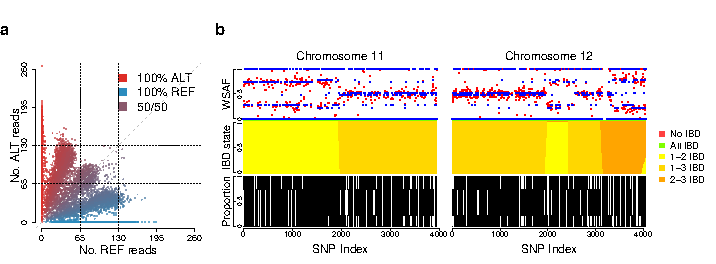
\includegraphics[width=\textwidth]{Fig1.pdf}
    \caption{Deconvolution of a complex field sample PD0577-C from Thailand.  (A) Scatter-plot showing the number of reads supporting the reference (REF: x-axis) and alternative (ALT: y-axis) alleles. The multiple clusters indicate the presence of multiple strains, but cannot distinguish the exact number or proportions.  (B) The profile of within-sample allele frequency along chromosomes 11 and 12 (red points) suggests a changing profile of IBD with three distinct strains, estimated to be with proportions of $22\%$, $52\%$ and $26\%$ respectively (other chromosomes omitted for clarity, see Figure~\ref{fig:fig1}-Supplement~1); blue points indicate expected allele frequencies within the isolate. However, the strains are inferred to be siblings of each other: green segments indicate where all three strains are IBD; yellow, orange and dark orange segments indicate the regions where one pair of strains are IBD but the others are not.  In no region are all three strains inferred to be distinct. (C) Statistics of  IBD tract length, in particular illustrating the N50 segment length. A graphical description of the modules and workflows for \texttt{DEploidIBD} is given in Figure~\ref{fig:fig1}-Supplement~2.}\label{fig:fig1}
  \end{center}

   \figsupp{Whole genome deconvolution of field sample PD0577-C. The outer ring shows the expected within-sample allele frequency (WSAF) (blue) and observed WSAF (red) across the genome. Red and blue points indicate observed and expected allele frequencies within the isolate. The inner ring indicates the IBD states among the three strains: green segments indicate where all three strains are IBD; yellow, orange and dark orange segments indicate the regions where one pair of strains are IBD but the others are not.  In no region are all three strains inferred to be distinct, suggesting that all three strains are siblings.}{\includegraphics[width=.7\textwidth]{{myring.ring}.pdf}}

   \figsupp{A graphical overview of the data types and work flows for \texttt{DEploidIBD}. The boxes at the bottom represent final outputs of the pipeline. The rectangular boxes indicate when \texttt{DEploidIBD} is executed, with inputs highlighted by blue arrows. The process has three key steps: Step 1. A reference panel for the set of samples is constructed from high confidence clonal haplotypes, either identified from within a study or from an external resource, such as Pf3k. Step 2: \texttt{DEploidIBD}, using population level allele frequencies, is used to infer the number of strains,  strain proportions and IBD profile within each sample. Step 3:  \texttt{DEploidIBD} is re-run on each sample to infer haplotypes, but with the proportions estimated in Step 2 fixed and this time using the haplotype (LD-aware) method previously implemented in \texttt{DEploid}.} {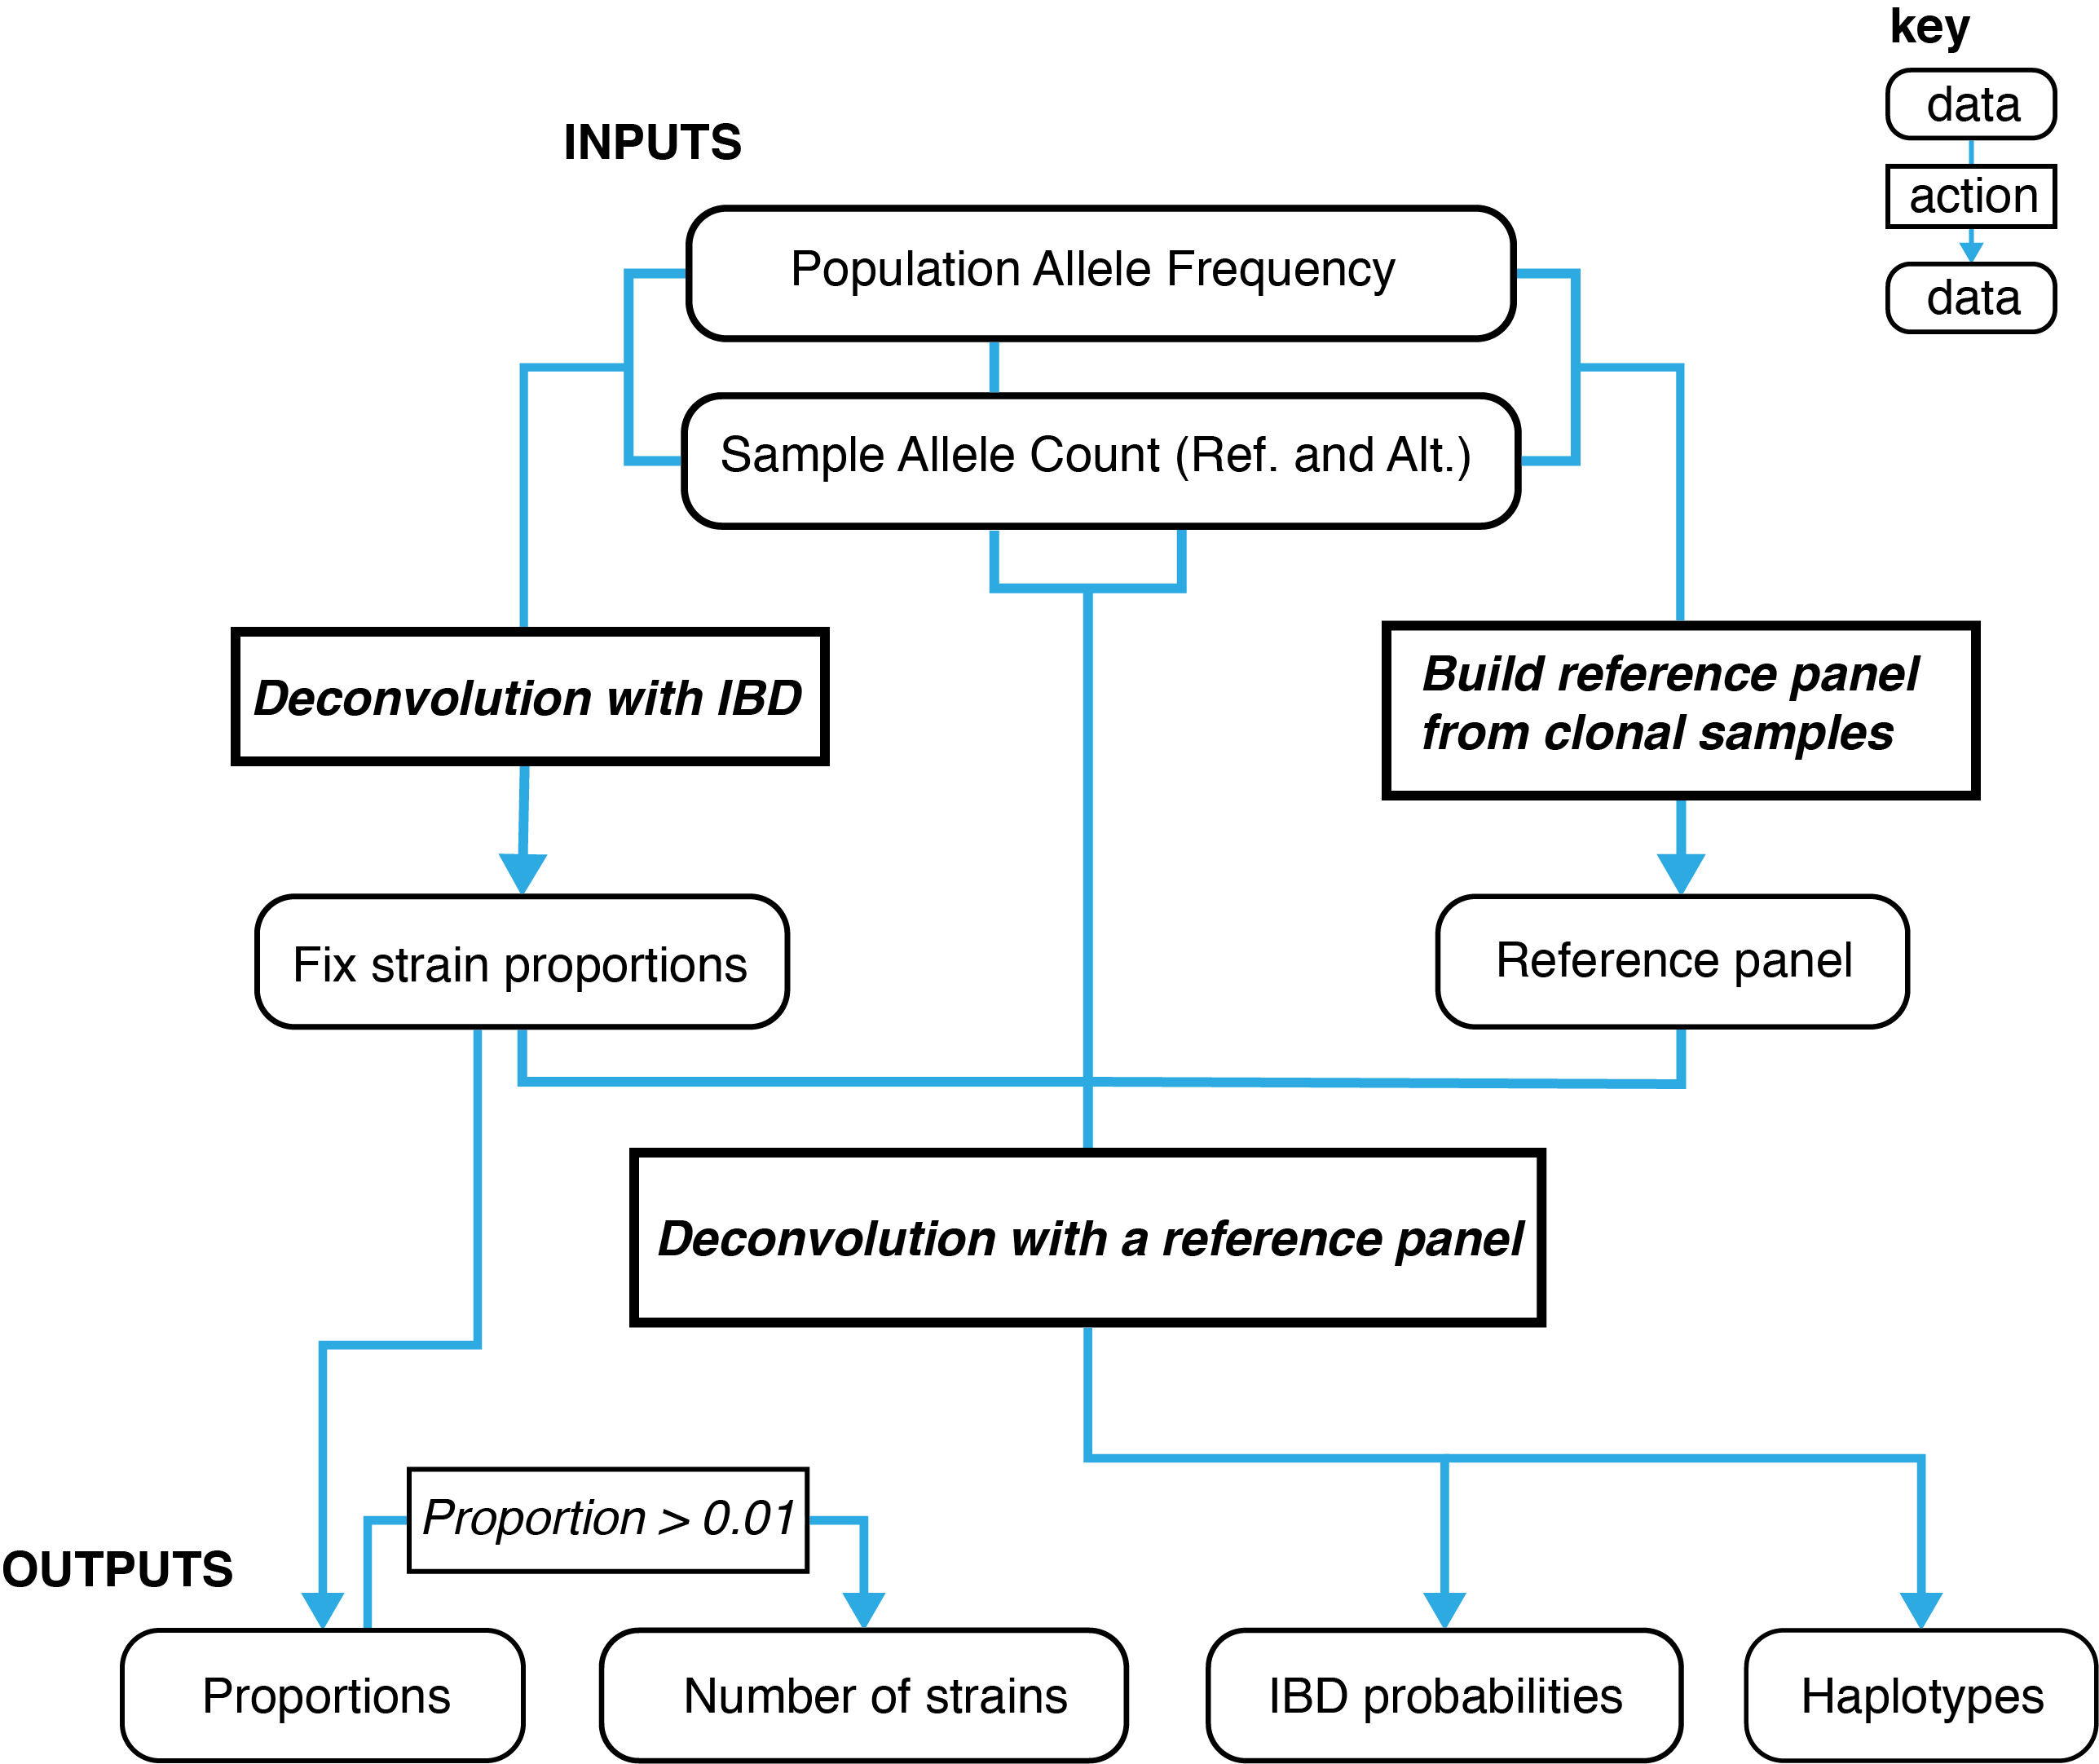
\includegraphics[width=.8\textwidth]{scheme-v2.png}}
\end{figure}




\section{Results}

\subsection{Method validation}

We validated \texttt{DEploidIBD} through both experimental mixtures using lab strains and {\it in silico} mixtures using clonal field samples.  First, to test consistency with \texttt{DEploid} \citet{Zhu2017}, we re-analysed the 27 experimental mixtures from \citep{Wendler2015}.  This data set includes 27 samples of various mixtures of four laboratory parasite lines (3D7, Dd2, HB3 and 7G8; Figure~\ref{fig:benchmark}--Supplement~3).  Allowing for mixtures of up to four strains and using optimal reference panels, we found comparable performance with the single-step \texttt{DEploid} method, with the exception of three strains of equal proportions where LD information is necessary to achieve accurate deconvolution (Figure~\ref{fig:benchmark}--Supplement~3).

To test the accuracy of \texttt{DEploidIBD} in a more realistic setting, we created {\it in silico} mixtures of two strains from 212 clonal samples of Asian origin (proportions ranging from 10/90\% to 45/55\%) using Chromosome 14 data (8,070 sites).  A further 20 randomly chosen samples were used as the reference panel. In order to compare the accuracy of the two methods at different levels of relatedness, we set 25\%, 50\% and 75\% of the second haplotype to be the same as the first haplotype to mimic scenarios of low, medium and high relatedness. This operation sets a lower limit to the relatedness between two samples. In a lower diversity region like Asia, because of the background relatedness, the actual relatedness is expected to be higher.  To simulate data, we used empirical read depths and drew read counts for the two alleles from binomial proportions.  We inferred strain proportions (summarised by the effective number of strains: $K_e = 1/\sum w_{i}^{2}$), and haplotypes. Both \texttt{DEploid} and \texttt{DEploidIBD} correctly estimate strain proportions with low relatedness (Figure~\ref{fig:benchmark}A). However, for moderate and high relatedness mixtures, \texttt{DEploid} fails to recover the correct proportion, when the minor strain proportion is below 30\%.

\texttt{DEploidIBD} is a substantial improvement on \texttt{DEploid}. In addition to estimating proportions and number of strains accurately in all settings, \texttt{DEploidIBD} estimates of relatedness and IBD tract length are  accurate.  Due to background relatedness {\tt DEploidIBD} typically over-estimates IBD fraction by a few percent  (Figure~\ref{fig:benchmark}B). Rates of genotype error are similar for the two approaches in settings of low relatedness (error rate of 0.4\% per site for 25/75 mixtures and 1.0\% for 45/55 mixtures).  However, for the 25/75\% mixtures with high relatedness, genotype error for the non-IBD approach increases to 0.6\%, while error in the IBD approach remains at 0.4\% (Figure~\ref{fig:benchmark}C). Switch errors in haplotype estimation are comparable between the two methods and decrease with increased relatedness due to the higher homozygosity (Figure~\ref{fig:benchmark}D). In summary, joint inference of IBD profiles and strain haplotypes is expected to improve estimates of strain proportions (and hence haplotypes), particularly in regions with high rates of IBD. Moreover, direct estimates of IBD within mixed infections can be used as an additional feature to characterise isolates.

\begin{figure}[htp]
  \begin{center}
  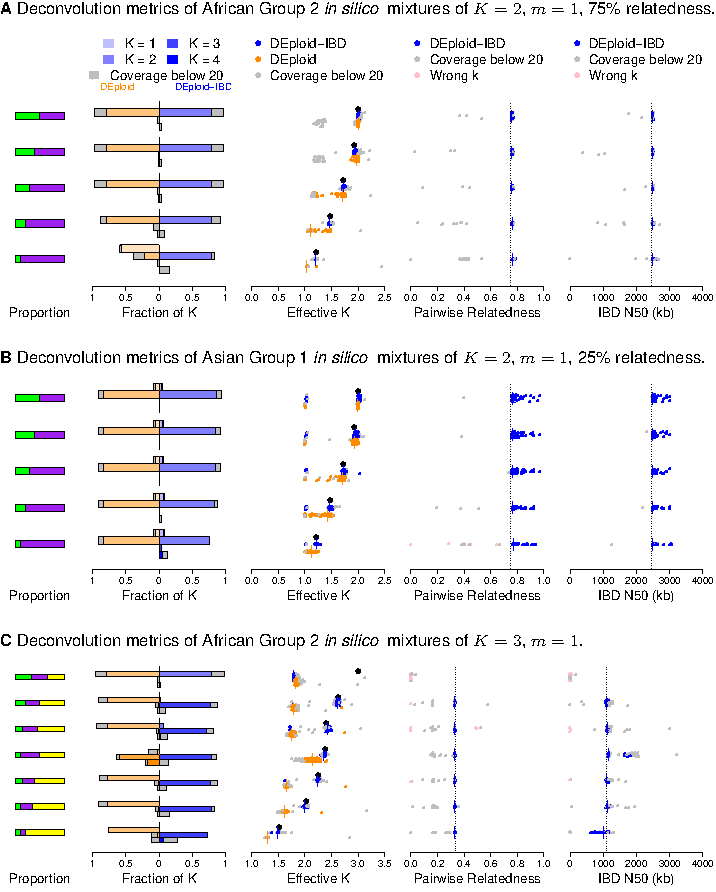
\includegraphics[width=.9\textwidth]{Fig2.pdf}
  \caption{Comparison of \texttt{DEploidIBD} and \texttt{DEploid}  on 76 {\it in silico} mixtures of two strains from Asia for 8,070 sites on Chromosome 14. (A) Relative differences of inferred effective number of strains using \texttt{DEploid} and \texttt{DEploidIBD}. The relative difference is calculated as the difference between inferred and expected effective number of strains divided by the expected value. (B) Inferred pairwise relatedness and N50 IBD tract length using \texttt{DEploidIBD}. Dotted lines indicate parameters used in the simulation. (C) Cumulative distribution of the average per site genotype error across simulated mixtures with three levels of IBD (25\%, 50\% and 75\%) for a mixture proportion of $25/75\%$. We performed 100 simulations, but excluded eight cases where simulated haplotypes were over 99\% identical and another 16 cases where average coverage was below 20.  (D) Cumulative distribution of haplotype switch errors with three levels of IBD (25\%, 50\% and 75\%) for a mixture proportion of 25$\slash$75\%.
  }\label{fig:benchmark}
  \end{center}

  \figsupp{Performance of \texttt{DEploidIBD} on 81 {\it in silico} mixtures of two strains from Africa using 92,780 sites from Chromosome 14. (A) Relative differences of inferred effective number of strains. (B) Inferred pairwise relatedness and N50 IBD tract length. Dotted lines mark parameters used in the simulation. (C) Cumulative distribution of average per site genotyping error for three levels of IBD (25\%, 50\% and 75\%).  (D) Cumulative distribution of haplotype switch error for the same three levels of IBD.
  }{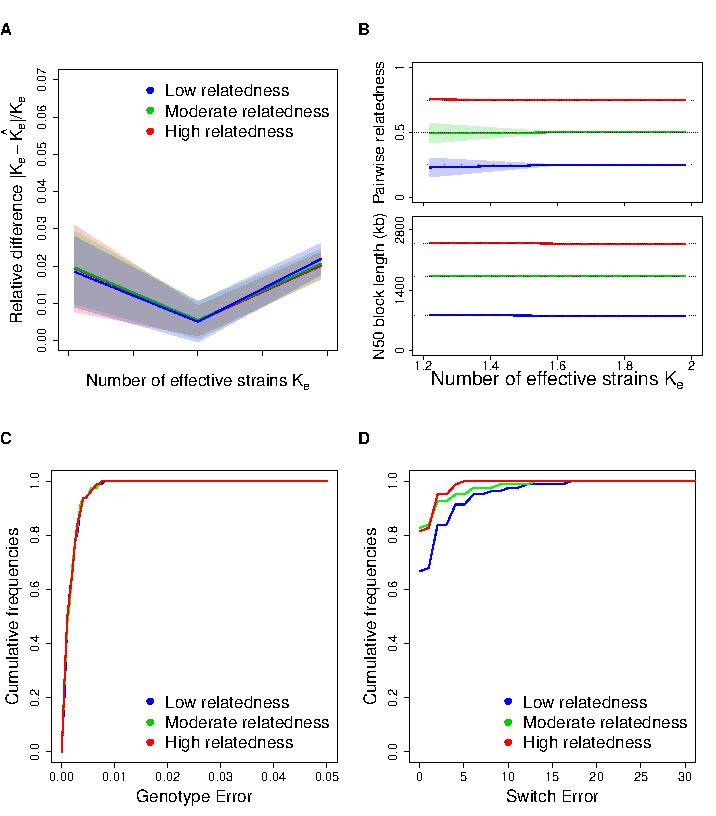
\includegraphics[width = \textwidth]{Fig2Africa.pdf}}
    \newcounter{fig2Counter}
    \setcounter{fig2Counter}{\value{enumi}}
  \end{figure}

\begin{figure}[ht]
  \setcounter{enumi}{\value{fig2Counter}}
  \setcounter{figsupp}{1}
  \figsupp{Performance of \texttt{DEploidIBD} and \texttt{DEploid} on {\it in silico} mixtures of three strains from Asia. $p_1$ and $p_2$ denote the proportions of the minor strains 1 and 2 respectively. The third strain, with proportion of $1-p_1-p_2$, always has the largest proportion. We consider two scenarios: five cases  with $p_1 = p_2$ in the range $0.1 \leq p_1 \leq 0.35$)  and 10 cases with $p_1<p_2$: (0.10, 0.15, 0.75), (0.10, 0.20, 0.70), (0.10, 0.25, 0.65), (0.15, 0.20, 0.65), (0.10, 0.30, 0.60), (0.15, 0.25, 0.60), (0.10, 0.40, 0.50), (0.15, 0.30, 0.55), (0.20, 0.25, 0.55) and (0.20, 0.30, 0.50). (A) Illustration of the mixture proportion profile over the effective $K$ surface. Let red and green color represent scenarios that $p_1 = p_2$ and $p_1 < p_2$. (B) Relative difference of inferred effective number of strains using \texttt{DEploid} and \texttt{DEploidIBD}. (C) Inferred pairwise relatedness and N50 IBD tract length. Dashed lengths indicate the tract lengths of the first and the second 50\% of the SNPs.}{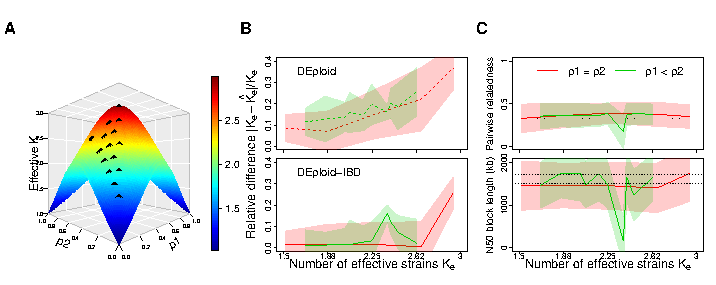
\includegraphics[width = \textwidth]{Fig2SupMix3.pdf}}

  \figsupp{Validation of {\tt DEploidIBD} using 27 experimental lab mixtures. A reference panel of the laboratory  strains (3D7, Dd2, HB3 and 7G8; Panel V) was used to deconvolve samples with {\tt DEploid}. Each experiment is performed with and without IBD inference and with two values of the maximum number of strains (3 and 4). Black crosses indicate the true effective number of strains. Coloured crosses indicate median values obtained from 30 replicates using the algorithm/strain number indicated in the legend. The coloured dots show the inferred effective number of strains across replicates with intensity proportional to fraction. Note one sample (indicated by an asterisk and dotted red line) where balanced proportions of three strains results in the LD-free approach fitting the data as a mixture of two strains with proportions of $1\slash3$ and $2\slash3$.}{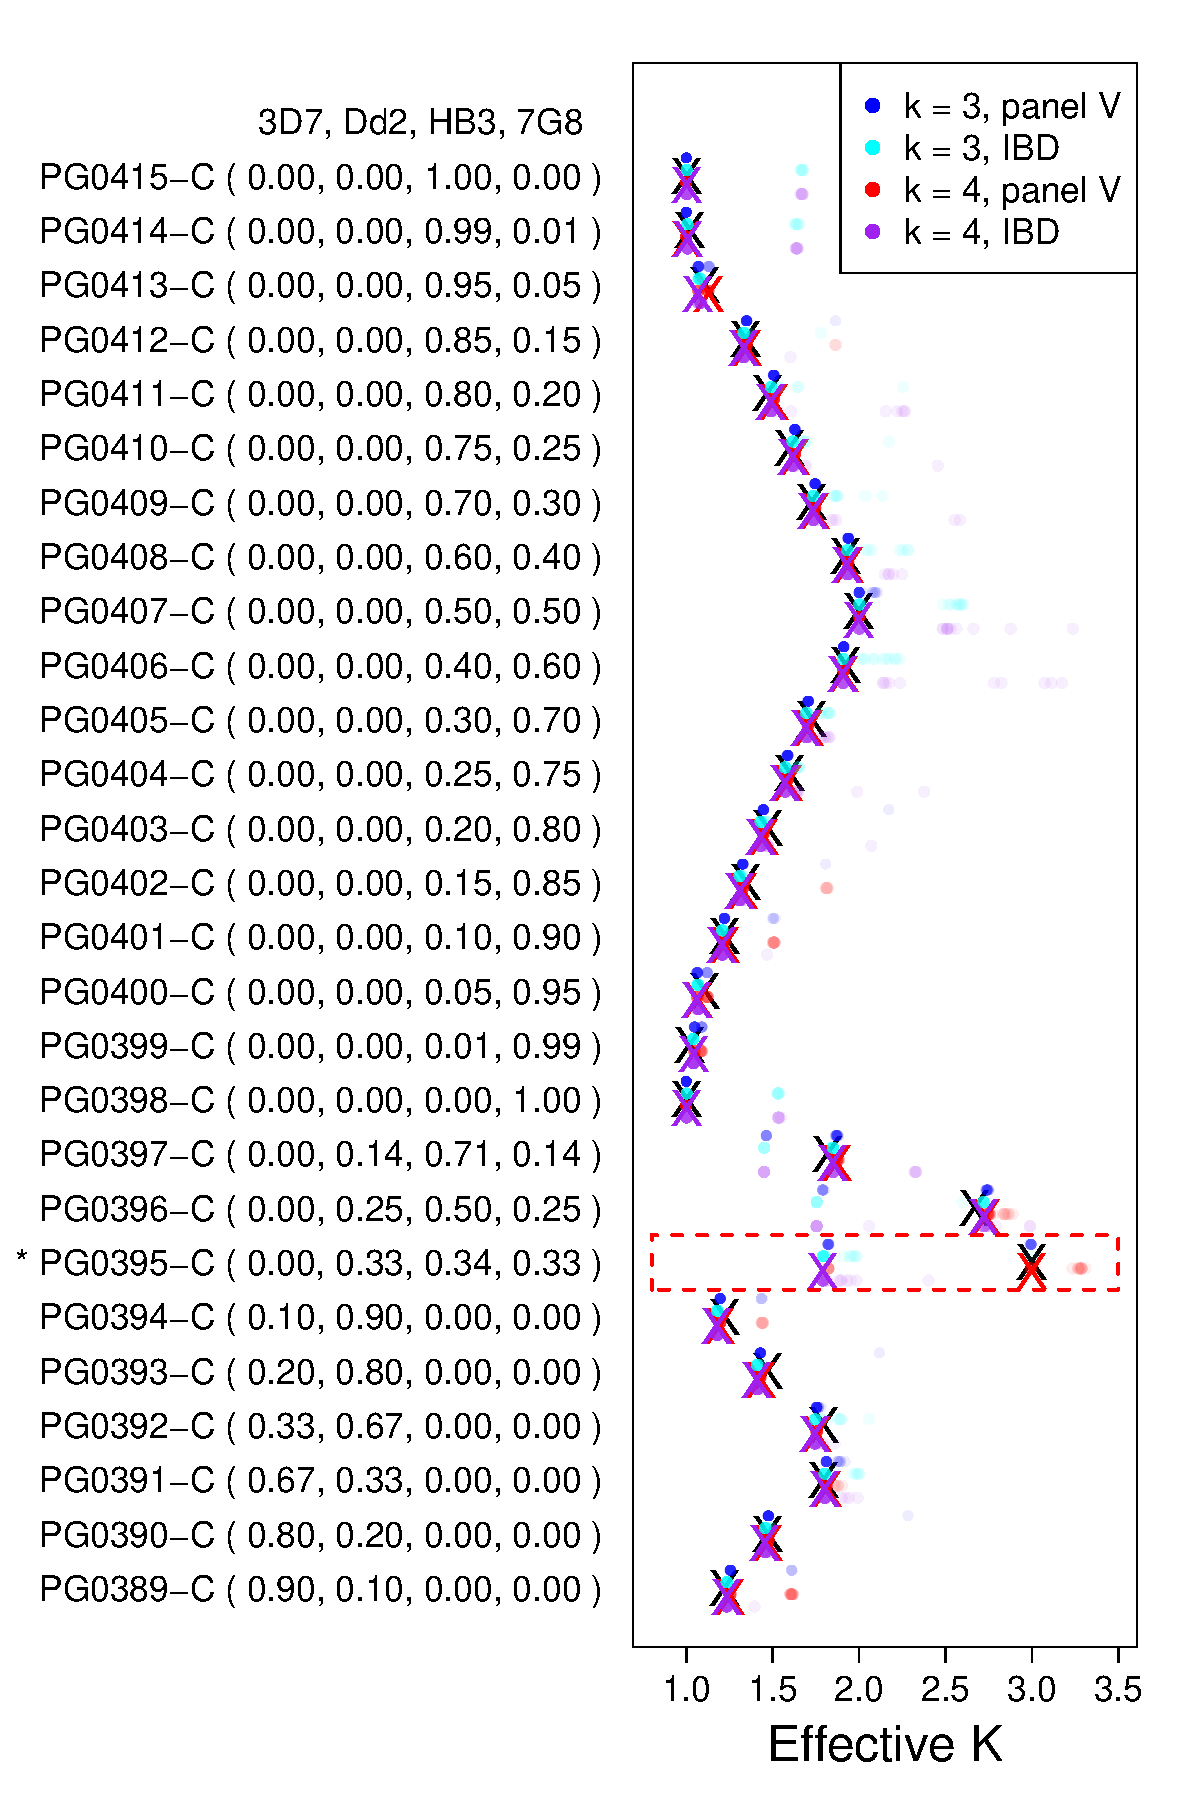
\includegraphics[width=0.6\textwidth]{eff_k_both.pdf}}
\end{figure}

We repeated the \emph{in silico} experiment with  mixtures of two strains from 197 clonal African samples, with mixing proportions of 10/90\%, 25/75\% and 45/55\%, using 92,780 sites from Chromosome 14. \texttt{DEploidIBD} estimates the correct proportions at all relatedness levels (Figure~\ref{fig:benchmark}--Supplement~1), although with a greater relative difference in effective $K$ compare to Asia ($\sim$ 2\% vs. $\sim$ 1\%). \texttt{DEploidIBD} also recovers the correct level of relatedness and IBD tract length (note that in Africa background relatedness is typically low). The per site genotype error rate remains below 1\%.  The number of haplotype switch errors is higher than in Asia, but by a factor much less than the 11-fold increase in the number of SNPs.

Finally, we extended benchmarking to \emph{in silico} mixtures of three Asian strains  (Figure~\ref{fig:benchmark}--supplement~2). We set one strain to have the highest proportion (the dominant strain) and constructed the two minor strains to be IBD with the dominant strain over distinct halves of the chromosome, such that at any point there are only two distinct haplotypes present.  We find that \texttt{DEploidIBD} outperforms (lower relative difference) \texttt{DEploid} in all cases and typically provides accurate estimates of proportions (Figure~\ref{fig:benchmark}--Supplement~2) with the exception of two cases. For the case of (0.10, 0.40, 0.50), the minor strain creates very weak allele frequency imbalance, leading {\tt DEploidIBD} to infer the number of strains as two (with proportions $sim 45/55\%$) in 90/100 cases. For the case of (0.30, 0.30, 0.40), the problem is fundamentally unidentifiable and \texttt{DEploidIBD} fits the data as a mixture of two strains.  In these cases, \texttt{DEploidIBD} also underestimates the pairwise relatedness and N50 tract lengths.


\subsection{Geographical variation in mixed infection rates and relatedness}

To investigate how the rate and relatedness structure of mixed infections varies among geographical regions with different epidemiological characteristics, we applied \texttt{DEploidIBD} to 2,344 field samples of {\it P. falciparum} released by the Pf3k project \citep{pf3k}.  These samples were collected under a wide range of studies with heterogeneous designs, with the majority of samples being taken from symptomatic individuals seeking clinical treatment. A summary of the data sources is presented in Table~\ref{tab:Pf3k} and full details regarding study designs can be found at \url{https://www.malariagen.net/projects/pf3k#sampling-locations}.  Details of data processing are given in the Methods. For deconvolution, samples were grouped into geographical regions by genetic similarity; four in Africa, and three in Asia. (Table~\ref{tab:Pf3k}). Reference panels were constructed from the clonal samples found at each region. Since previous research has uncovered severe population structure in Cambodia \citep{Miotto2013}, we stratified samples into West and North Cambodia when performing analysis at the country level. Diagnostic plots for the deconvolution of all samples can be found at \url{https://github.com/mcveanlab/mixedIBD-Supplement} and inferred haplotypes can be accessed at URL.  We identified 787 samples where low sequencing coverage or the presence of low-frequency strains resulted in unusual haplotypes (see Supplementary Material).  Estimates of strain number, proportions and IBD states from these samples are used in subsequent analyses, but not the haplotypes.  We also confirmed that reported results are not affected by the exclusion of all metrics from samples with poor haplotypes.


\begin{table}[btp]
  \caption{Summary of Pf3k samples.}\label{tab:Pf3k}
{\small
\begin{tabular}{p{1.3cm} c p{1.8cm} c | c c c c p{2.7cm}}
\toprule\hline
                %&                    &      &         &        &                   &              &          &  \\
Country         &   Year  &Location  & $PfPr$ & $ss$   & $\bar{D}$ (s.e.)  & $\bar{\rho}$ & $\bar{K}$& Reference\\
\midrule
Gambia          &    2008 & Brikam   & 0.06   & 65     & 129 ( 9.4 )  & 0.53 & 1.3 &\citet{Amambua-Ngwa2012}\\
\hline
Ghana           &    2009 & Kassena & 0.79 & 121 & 86 ( 5.7 )& 0.25 & 1.6&\multirow{3}{*}{\parbox{3.4cm}{\citet{Duffy2015,Kamau2015,eLife2016}}}\\
                & 2010 & Kassena & 0.79 & 171 & 127 ( 10.3 )& 0.26 & 1.5 &\\
                & 2011 & Kassena & 0.72 & 97 & 76 ( 5.3 )& 0.24 & 1.5& \\
                &      & Kintampo & 0.58 & 6 & 89 ( 13.5 )& 0.16 & 1.5&\\
                & 2012 & Kassena & 0.52 & 47 & 111 ( 3.8 )& 0.31 & 1.6&\\
                &      & Kintampo & 0.41 & 40 & 157 ( 8.1 )& 0.25 & 1.6&\\
                & 2013 & Kassena & 0.31 & 88 & 119 ( 4 )& 0.29 & 1.6&\\
                &      & Kintampo & 0.29 & 4 & 172 ( 38.4 )& 0.53 & 1.1&\\
\hline
Malawi & 2011 & Chikwawa & 0.19 & 230 & 101 ( 3 )& 0.28 & 1.7 &\citet{Ocholla2014}\\
       &      & Zomba & 0.34 & 35 & 89 ( 9.1 )& 0.28 & 1.6 &\\
\hline
Mali & 2007 & Bandiagara & 0.43 & 9 & 95 ( 25.2 )& 0.39 & 1.8  &\multirow{3}{*}{\parbox{3.4cm}{\citet{eLife2016}}}\\
     &      & Faladje & 0.37 & 36 & 75 ( 10.1 )& 0.34 & 1.3 &\\
     &      & Kolle & 0.21 & 51 & 82 ( 10.5 )& 0.36 & 1.6 &\\
\cline{1-8}
Guinea & 2011 & Nzerekore & 0.49 & 97 & 77 ( 4.6 )& 0.21 & 1.4 &\\
\cline{1-8}
Congo DR        & 2013 & Kinshasa & 0.24 & 113 & 49 ( 3.2 )& 0.36 & 1.5\\
\hline
Senegal & 2004 & Thies & 0.09 & 2 & 130 ( 68.2 )& 0.03 & 1.4  &\citet{Wong2017}\\
        & 2009 & Thies & 0.04 & 43 & 175 ( 14.9 )& 0.47 & 1.1  &\\
        & 2010 & Thies & 0.04 & 24 & 159 ( 9.7 )& 0.36 & 1.3 &\\
        & 2011 & Thies & 0.03 & 32 & 97 ( 6 )& 0.4 & 1.1 &\\
\hline
\hline
West     & 2009 & Pursat & 0.0071 & 19 & 75 ( 8.8 )& 0.39 & 1.3 &\multirow{3}{*}{\parbox{3.4cm}{\citet{Amato2017, eLife2016}}}\\
Cambodia & 2010 & Pursat & 0.0071 & 105 & 95 ( 6.8 )& 0.65 & 1.2&\\
         & 2011 & Pailin & 0.0025 & 49 & 54 ( 4.1 )& 0.43 & 1.1&\\
         &      & Pursat & 0.0096 & 103 & 49 ( 3.1 )& 0.63 & 1.2&\\
         & 2012 & Pailin & 0.00096 & 31 & 46 ( 5.6 )& 0.43 & 1.0&\\
         &      & Pursat & 0.0079 & 7 & 37 ( 19.1 )& 0.58 & 1.4&\\
\cline{1-8}
North & 2010 & Ratanakiri & 0.0039 & 50 & 71 ( 6.1 )& 0.44 & 1.3&\\
Cambodia  & 2011 & Preah Vihear & 0.02 & 73 & 51 ( 5.3 )& 0.36 & 1.2&\\
          &      & Ratanakiri & 0.0032 & 81 & 45 ( 4.3 )& 0.48 & 1.4&\\
          & 2012 & Preah Vihear & 0.0075 & 30 & 43 ( 6.7 )& 0.38 & 1.0&\\
          &      & Ratanakiri & 0.0016 & 15 & 44 ( 8.9 )& 0.32 & 1.3&\\
\hline
Thailand & 2011 & Mae Sot & 0.00011 & 35 & 66 ( 7.5 )& 0.35 & 1.2 &\multirow{3}{*}{\parbox{3.4cm}{\citet{Miotto2013, eLife2016}}}\\
         &      & Sisakhet & 1e-04 & 5 & 112 ( 25.4 )& 0.17 & 1.3 &\\
         & 2012 & Mae Sot & 5.7e-05 & 69 & 83 ( 4.9 )& 0.59 & 1.3 &\\
         &      & Ranong & 0.00018 & 11 & 82 ( 12.4 )& 0.34 & 1.2 &\\
         &      & Sisakhet & 0 & 13 & 89 ( 13 )& 0.37 & 1.1 &\\
         & 2013 & Sisakhet & 0 & 3 & 62 ( 8.8 )& 0.09 & 1.2&\\
\cline{1-8}
Bangladesh & 2012 & Ramu & 0.0021 & 50 & 53 ( 4.2 )& 0.49 & 1.5 &\\
\cline{1-8}
Viet Nam & 2011 & Bu Gia Map & 0.0073 & 43 & 67 ( 5 )& 0.44 & 1.3&\\
         &      & Phuoc Long & 0.0053 & 27 & 68 ( 7.2 )& 0.38 & 1.2&\\
         & 2012 & Bu Gia Map & 0.0072 & 19 & 115 ( 8 )& 0.67 & 1.1&\\
         &      & Phuoc Long & 0.0048 & 5 & 107 ( 6.3 )& 0.82 & 1.2&\\
\cline{1-8}
Myanmar & 2011 & Bago Division & 0.0076 & 12 & 59 ( 7.1 )& 0.26 & 1.2 &\\
        & 2012 & Bago Division & 0.0084 & 47 & 62 ( 5.2 )& 0.46 & 1.2 &\\
\cline{1-8}
Laos & 2011 & Attapeu & 0.0094 & 59 & 71 ( 4.2 )& 0.37 & 1.4 &\\
     & 2012 & Attapeu & 0.02 & 25 & 77 ( 7.2 )& 0.69 & 1.3 &\\
\hline
\bottomrule
\end{tabular}
}

\tabledata{Summary of Pf3k samples in data release 5.1, where $D$ denotes mean read depth and $ss$ is sample size.  Genotyping, including both indel and SNP variants, was performed using a pipeline based on GATK best practices, see Methods. Data available from \url{ftp://ngs.sanger.ac.uk/production/pf3k/release_5/5.1}. $PfPr$ is the inferred parasite prevalence rate in a 5 $\times$ 5 km resolution grid from the MAP project, centred at the Pf3k sample collection sites; Relatedness $\rho$ and effective number of strains $K$ are summary metrics from {\tt DEploidIBD} output.}
\end{table}



We find substantial variation in the rate and relatedness structure of mixed infections across continents and countries.  Within Africa, rates of mixed infection vary from 18\% in Senegal to 63\% in Malawi (Figure~\ref{fig:mixInfPlot}A). In Southeast Asian samples, mixed infection rates are in general lower, though also vary considerably; from 21\% in Thailand to 54\% in Bangladesh.  Where data for a location is available over multiple years, we find no evidence for significant fluctuation over time (though we note that these studies are typically not well powered to see temporal variation and collection dates are very heterogeneous). We observe that between 5.1\% (Senegal) and 40\% (Malawi) of individuals have infections carrying more than two strains.

\begin{figure}[ht]
  \begin{center}
    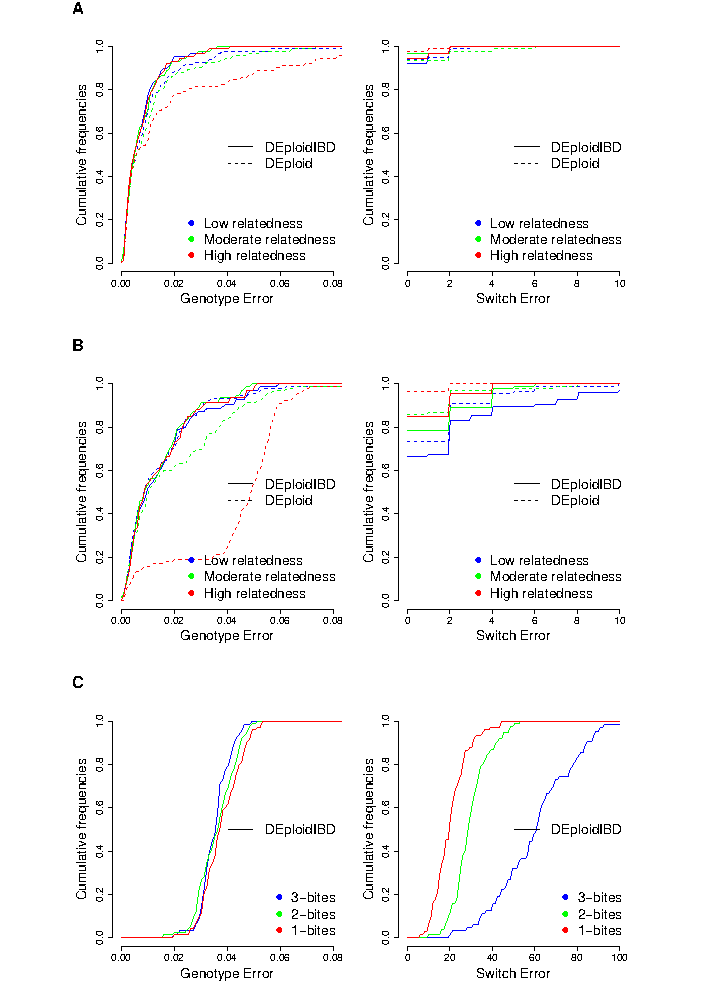
\includegraphics[width=\textwidth]{Fig3.pdf}
    \caption{Characterisation of mixed infections across 2,344 field samples of {\it Plasmodium falciparum}. (A) The fraction of samples, by population, inferred to carry one (clonal), two, three, or more than three strains.  Populations are ordered by rate of mixed infections within each continent. We use shaded regions to indicate the distribution of 787 samples that have low-confidence deconvolved haplotypes.  (B) The distribution of IBD within mixed infections (including dual, triple and quad infections), broken down into unrelated (where the fraction of the genome inferred to be IBD, $r$, is $< 0.1$), low IBD ($0.1 \geq r < 0.3)$, sib-level ($0.3 \geq r<0.7$) and high ($r \geq 0.7$). Stars indicate the average IBD scaled between 0 and 1 from bottom to the top.  Populations follow the same order as in Panel A.  (C) The relationship between the rate of mixed infection and level of IBD. Populations are coloured by continent, with size reflecting sample size and error bars showing $\pm 1$ s.e.m..  The dotted line shows the slope of the regression from a linear model.  Abbreviations: SN-Senegal, GM-The Gambia, NG-Nigeria, GN-Guinea, CD-The Democratic Republic of Congo, ML-Mali, GH-Ghana, MW-Malawi, MM-Myanmar, TH-Thailand, VN-Vietnam, KH-Cambodia, LA-Laos, BD-Bangladesh.} \label{fig:mixInfPlot}
  \end{center}
\end{figure}

Relatedness between samples and populations also varies substantially.  In dual infections, the average fraction of the genome inferred to be IBD ranges from 21\% in Guinea to 59\% in West Cambodia (Figure~\ref{fig:mixInfPlot}B).  Asian populations show, on average, a higher level of relatedness within dual infections (48\%) compared to African populations (29\%).  Levels of IBD in samples with three or more strains are comparable to those seen in dual infections (average IBD being 50\% in Asia and 29\% in Africa) and significantly correlated at the country level (P = 0.0012), except Senegal.  Overall, 53\% of all mixed infections involve strains with over 30\% of the genome being IBD.

We next considered the relationship between mixed infection rate and the level of IBD.  We find that populations with higher rates of mixed infection tend to have lower levels of IBD in mixed infections (linear model P = 0.06 after accounting for a continental level difference and weighted by sample size).  However, the continental level effect is driven by Senegal, which has an unusual combination of low mixed infections and also low IBD.  Excluding Senegal, we find a consistent pattern across populations (Figure~\ref{fig:mixInfPlot}C), with a strong negative correlation between mixed infection rate and the level of IBD (Pearson $r = XXX$, P = $3\times10^{-4}$).  Previous work has demonstrated how a recent and dramatic decline in {\emph P. falciparum} prevalence within Senegal has left an impact on patterns of genetic variation \citep{Daniels2015}, which may explain its unusual profile.

\begin{figure}[ht]
  \begin{center}
  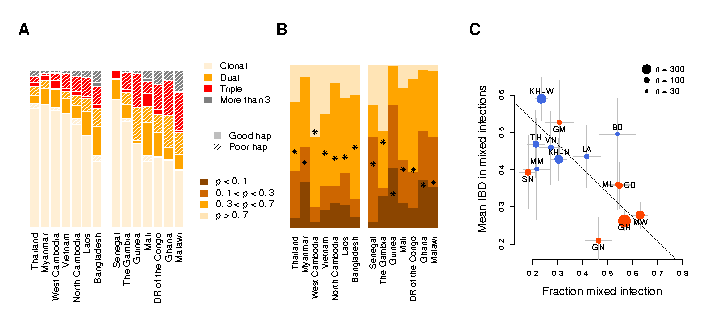
\includegraphics[width=.9\textwidth]{Fig4.pdf}
    \caption{Example IBD profiles in mixed infections. Plots showing the ALT versus REF plots (left hand side) and inferred IBD profiles along the genome for five strains of differing composition.  From top to bottom: A dual infection of highly related strains ($r = 0.84$); a dual infection of two sibling strains ($r = 0.6$); a triple infection of three sibling strains (note the absence of stretches without IBD); a triple infection of two related strains and one unrelated strain; and a triple infection of three unrelated strains.  The numbers below the sample IDs indicate the average pairwise IBD, $r$, and the mean length of IBD segments, $l$, respectively.}\label{fig:strainIBD}
    \end{center}
\end{figure}




\subsection{Inferring the origin of IBD in mixed infections}

The high levels of IBD observed in many mixed infections suggest the presence of sibling strains (Figure~\ref{fig:strainIBD}). To quantify the expected IBD patterns between siblings, we developed a meiosis simulator for {\it P. falciparum} ({\tt pf-meiosis}), incorporating relevant features of malaria biology that can impact the way IBD is produced in a mosquito and detected in a human host. Most importantly, a single infected mosquito can undergo multiple meioses in parallel, one occurring for each oocyst that forms on the mosquito midgut.  In a mosquito infected with two distinct strains, each oocyst can either self (the maternal and paternal strain are the same) or outbreed (the maternal and paternal strains are different). We model a $K = n$ mixed infection as a sample of $n$ strains (without replacement, as drawing identical strains yields $K = n-1$) from the pool of strains created by all oocysts. Most studies suggest that the distribution of oocysts is roughly geometric with a mean of 1.5, implying that the most common number of oocysts in an infected mosquito is one. Unexpectedly, in such a case, a $K=2$ infection will have an expected IBD of $1/3$. Conditioning on at least one progeny from an outbred oocyst (such that a detectable recombination event has occurred), the expected IBD asymptotically approaches $1/2$ as the total number of oocysts grows.

Using this simulation framework, we sought to classify observed mixed infections based on their patterns of IBD. We used two summary statistics to perform the classification: mean IBD segment length and IBD fraction. We built empirical distributions for these two statistics for each country in Pf3k, by simulating meiosis between pairs of clonal samples from that country.  In this way, we control for variation in genetic diversity (as background IBD between clonal samples) in each country. Starting from a pair of clonal samples ($M=0$, where $M$ indicates the number of meioses that have occurred), we simulated three successive rounds of meiosis ($M=1, 2, 3$), representing the creation and serial transmission of a mixed infection (Figure~\ref{fig:classify}A). Each round of meiosis increases the amount of observed IBD. For example, in Ghana, the mean IBD fraction for $M=0$ was 0.002, for $M=1$ was 0.41, for $M=2$ was 0.66, and for $M=3$ was 0.80 (Figure~\ref{fig:classify}B). West Cambodia, which has lower genetic diversity, had a mean IBD fraction of 0.08 for $M=0$ and consequently, the mean IBD fractions for higher values of $M$ were slightly increased, to 0.46, 0.68, 0.81 for $M=1, 2$ and $3$, respectively (Figure~\ref{fig:classify}B).

From these simulated distributions, we used Naive Bayes to classify all $k=2$ mixed infections in Pf3k (Figure~\ref{fig:classify}C).  Of the 404 samples with $K = 2$, 288 (71\%) had IBD statistics that fell within the range observed across all simulated $M$. Of these, more than half (221, 55\%) of all $K=2$ mixed infections were classified as siblings ($M > 0$, with > 99\% posterior probability).  Moreover, we observe geographical differences in the rate at which sibling and unrelated mixed infections occur. Notably, in Asia, a greater fraction of all mixed infections contained siblings (65\% vs. 51\% in Africa), driven by a notably higher frequency of $M=2$ and $M=3$ mixed infections (Figure~\ref{fig:classify}D).

\begin{figure}[htp]
  \begin{center}
  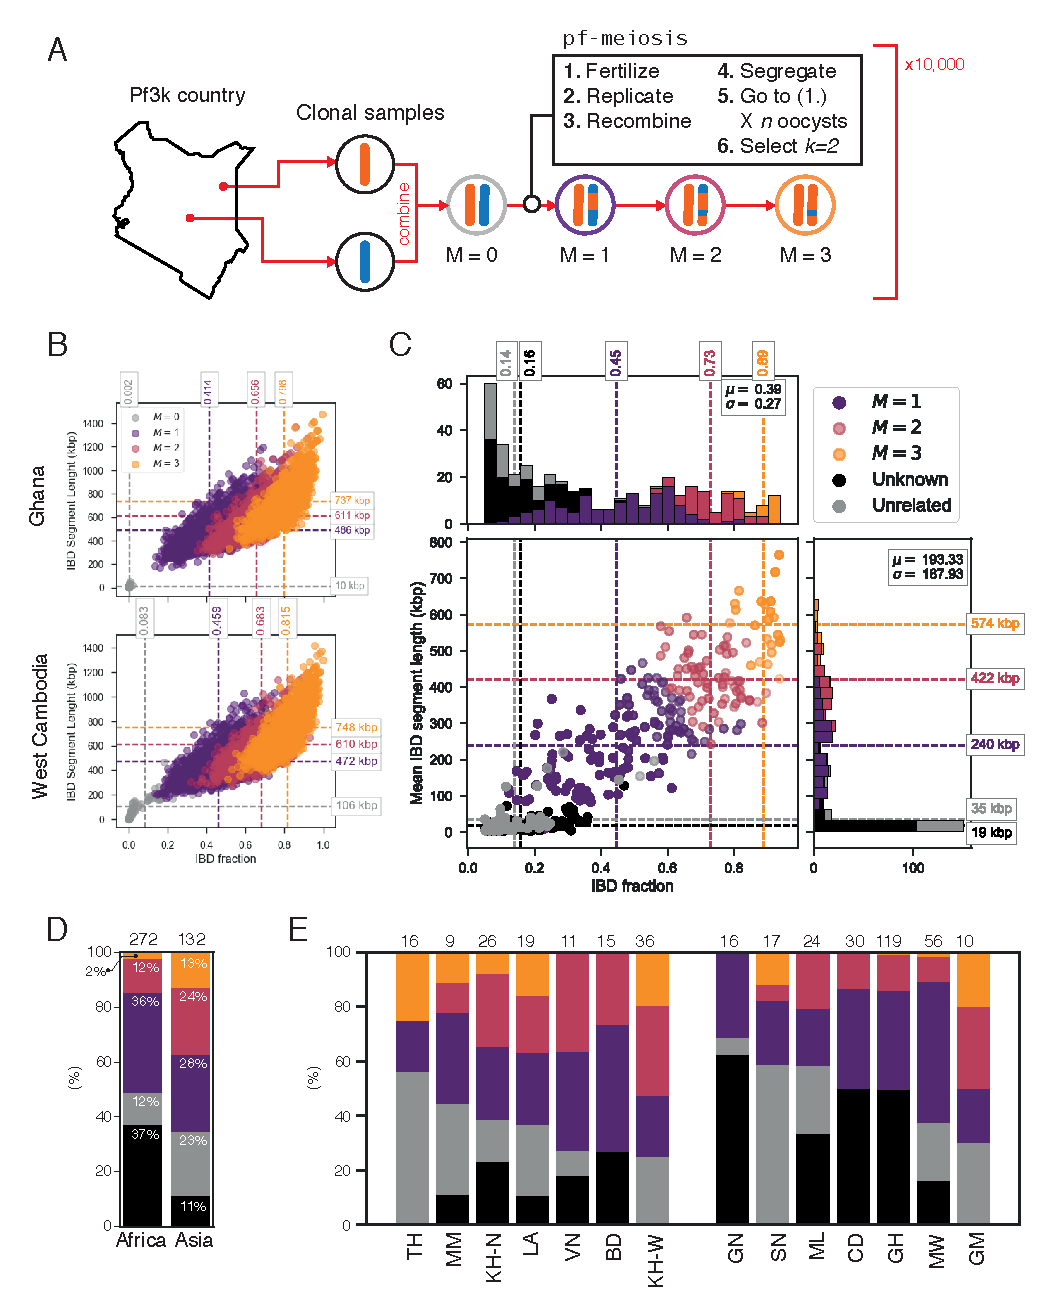
\includegraphics[width=\textwidth]{Fig4-v3.pdf}
   \caption{Identifying sibling strains within mixed infections.  (A) Generating IBD fraction and segment length distributions for unrelated ($M=0$, grey), sibling ($M=1$, purple), inbred-sibling ($M=2$, pink) and doubly-inbred-sibling ($M=3$, orange) mixed infections. Two clonal samples from a given country are combined to produce a $K=2$ unrelated mixed infection which recapitulates local background IBD. This unrelated infection is then passed through $n$ rounds of \tt{pf-meioses} a malaria-specific meioses simulator, to generate $M=n$ classes. (B) Simulated IBD distributions for $M=0...3$ for Ghana and West Cambodia. A total of 10,000 progeny are simulated for each class (C) Classification result for 404 $K=2$ mixed infections from 14 countries. Unknown indicates mixed infections with IBD statistics that were never observed in simulations. (D) Breakdown of class percentage by continent. Total number of samples is given above bars. (E) Breakdown of class percentage by country. Abbreviations as in Figure \ref{fig:mixInfPlot}.}
   \label{fig:classify}
   \end{center}
\end{figure}



\subsection{Characteristics of mixed infections correlate with local parasite prevalence}

To assess how characteristics of mixed infection relate to local infection intensity, we obtained estimates of {\it P. falciparum} prevalence (Pfpr) from the Malaria Atlas Project \citep[see Table~\ref{tab:Pf3k}]{MAP2017}. The country level prevalence estimates range from 0.01\% in Thailand to 55\% in Ghana, with African countries having up to two orders of magnitude greater average infection intensity (mean of 36\% in Africa and 0.6\% in Asia). However, seasonal and geographic fluctuations in prevalence mean that, conditional on sampling an individual with malaria, local prevalence may be much higher than the longer-term (and more geographically widespread) average. We summarise mixed infection rates by the average effective number of strains, which reflects both the number and proportion of strains present.  This metric both avoids the problem of having to determine a threshold for determining the presence of a very low proportion strain and is sensitive to the presence of triply (and more) infected samples.

We find that the effective number of strains is a significant predictor of Pfpr within African populations ($r=0.48, P=XXX$), but is uncorrelated within Asian populations. Similarly, within-sample IBD and background IBD are both negatively correlated with PfPr only within Africa ($r= -0.67, P=XXX$ and $r = -0.53, P=XXX$, respectively).  The rate of sibling infection is strongly related to within-sample IBD and shows a similar relationship to Pfpr.  Interestingly, all statistics relating to IBD are positively correlated with Pfpr in Asian populations (though not significantly so), in contrast to the negative (and significant) associations seen within African populations.  



\begin{figure}[ht]
  \centering{}
  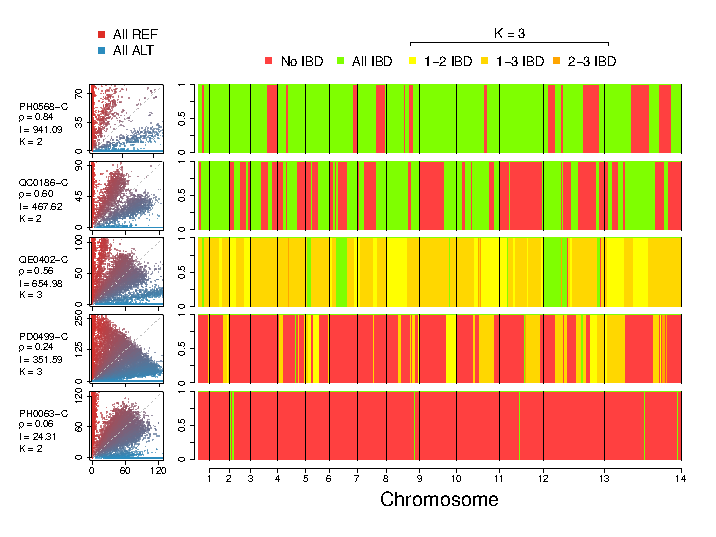
\includegraphics[width=\textwidth]{Fig5.pdf}
  \caption{The relationship between {\it P. falciparum} prevalence (Pfpr) and characteristics of mixed infection including (A) the average effective number of strains, given by $K_e = (\sum w_i^2)^{-1}$, where $w_i$ is the proportion of the $i$th strain; (B) within sample relatedness (average IBD fraction) in mixed samples; (C) background relatedness between clonal samples; and (D) super sibling rate in dual infections. Each point relates to a row in Table~1 from different sampling locations and years. Point size is proportional to Pf3k sample size. }
  \label{fig:model}
\end{figure}



\section{Discussion}

It has long been appreciated that mixed infections are an integral part of malaria biology, determining the number, proportions and haplotypes of the strains that comprise them, has proven a formidable challenge.  Previously we developed an algorithm, \texttt{DEploid}, for deconvolving mixed infections \citep{Zhu2017}.  However, we subsequently noticed the presence of mixed infections with highly related strains in which the algorithm performed poorly, particularly with low-frequency minor strains.  Mixed infections containing highly related strains represent an epidemiological scenario of particular interest, because  they are likely to have been produced from a single mosquito bite, itself multiply infected, and in which meiosis has occurred to generate sibling strains. Thus, we developed an enhanced method, \texttt{DEploidIBD}, capable not only of deconvolving highly related mixed infections, but also providing a profile of that IBD segments between all pairs of strains present in the infection.  We note that technical difficulties remain, including analysing data with multiple infecting species, coping with low-coverage data and selecting appropriate reference panels from the growing reference resources. 

The application of \texttt{DEploidIBD} to the 2,344 samples in the Pf3k project has revealed the extent and structure of relatedness among malaria infections and how these characteristics vary between geographic locations. We found that 1,026 (44\%) of all samples in Pf3k were mixed, being comprised of 505 $K=2$ infections, 374 $K=3$ and 147 $K=4$ infections. Across the entire data set, the total number of genomes extracted from mixed infections is more than double the number extracted from clonal infections (2,720 genomes from $K>1$ vs. 1,318 from $K=1$).  We also found  considerable variation, between countries and continents in the characteristics of mixed infections, suggesting that they are sensitive to local epidemiology.  For example, in West Africa, Senegal (which has undergone a recent and effective malaria control campaign) has a rate of mixed infections less than half that of neighbouring Guinea and Mali.  Previous work has highlighted the utility of mixed infection rate in discerning changes in regional prevalence, and we re-enforce that finding here, observing a significant correlation between the effective number of strains and parasite prevalence across Pf3k collection sites. Similarly, using \texttt{DEploidIBD} we also observe significant geographical variation in the relatedness profiles of strains within mixed infections.  Interestingly, this variation is structured such that regions with high rates of mixed infection tend to contain strains that are less related, resulting in a significant negative correlation between mixed infection rate and mean relatedness within those infections.

The ability to identify the extent and genomic structure of IBD enables inference of the mechanisms by which mixed infection can arise.  A mixed infection of $K$ strains can be produced by either $K$ independent infectious bites or by $j < K$ infectious bites. In the first case, parasites are delivered by separate vectors and no meiosis occurs, thus any IBD observed in the mixed infection must have pre-existed as background IBD between the individual strains.  In the second case, meiosis may occur between parasite strains, resulting in long tracts of IBD.  The exact amount of IBD produced by meiosis is a random variable, dependent on outcomes of meiotic processes, such as the number of and distance between recombination events and the segregation of chromosomes, as well as background IBD.  Importantly, the mean IBD produced during meiosis in \textit{P. falciparum} also depends on the number and type (selfed vs outbred) of oocysts in the infectious mosquito.  Consequently, the amount of IBD expected in a single-bite mixed infection produced from two unrelated parasites strains will always be slightly less than $1/2$, and as low as $1/3$.

To quantify the distribution of IBD statistics expected through different mechanisms of mixed infection we developed a Monte Carlo simulation tool, \texttt{pf-meiosis}, which we used to infer the recent transmission history of  individuals with dual ($K=2$) infections.  We considered mixed infection chains, in which $M$ successive rounds of meiosis, transmission to host and uptake by vector can result in sibling strain infections with very high levels of IBD.  Overall, we found that 56\% of all mixed infections are from sibling strains and, particularly within Asian population samples, evidence for long mixed infection chains ($M>1$).  This observation is not a product of lower genetic diversity in Asia, as differences in background IBD between countries have been controlled for in the simulations. Rather, it reflects true differences in transmission epidemiology between continents. These findings have three important consequences.  First, it suggests that successful establishment of multiple strains through a single infection event is major source of mixed infection.  Second, it implies that the bottlenecks imposed at transmission (to host and vector) are relatively weak.  Finally, it indicates that the source of mixed infections reflects aspects of local epidemiology.

We note that a non-trivial fraction (XX\%) of all mixed infections had patterns of IBD inconsistent with the simulations (typically higher IBD than background but lower than among sibs).  We suggest two explanations.  Firstly, our estimate of background IBD, generated by combining pairs of random clonal samples from a given country into an artificial $M=0$ mixed infection, will underestimate true background IBD if there is very strong local population structure.  Second, we only simulated simple mixed infection transmission chains, at the exclusion of more complex transmission histories, such as involving strains related at the level of cousins. The extent to which such complex histories can be inferred with certainty remains to be explored.

Finally, our results show that the rate and relatedness structure of mixed infection correlate with estimated levels of pathogen transmission intensity, at least within Africa, where prevalence is typically high and relatively stable over seasons.  In Asia, which has much lower overall transmission, as well as greater temporal (and possibly spatial) fluctuations in transmission intensity, we do not see such correlations.  However, it may well be that genomic features of the pathogen can provide much higher resolution in space and time for capturing changes in prevalence, than traditional methods.  Testing this hypothesis will lead to a much greater understanding of how genomic data can potentially be used  to inform global efforts to control and eradicate malaria.


\section{Methods and Materials}

The data analysed within this paper were collected and made openly available to researchers by member of the Pf3k Consortium.  Information about studies within the data set can be found at \url{https://www.malariagen.net/projects/pf3k#sampling-locations}.  Detailed information about data processing can be found at \url{https://www.malariagen.net/data/pf3k-5}.  Briefly, field isolates were sequenced to an average read depth of 86 (range 12.6 -- 192.5).  After removing human-derived reads and mapping to the 3D7 reference genome, variants were called using GATK best practice and approximately one million variant sites were genotyped in each isolate. After filtering samples for low coverage and cross-species contamination, 2,344 samples remained.    The Supplementary Material provides details on the filters used and data availability. For deconvolution, samples were grouped into geographical regions by genetic similarity; four in Africa, and three in Asia. (Table~\ref{tab:Pf3k}). Reference panels were constructed from the clonal samples found at each region. Since previous research has uncovered severe population structure in Cambodia \citep{Miotto2013}, we stratified samples into West and North Cambodia when performing analysis at the country level. Diagnostic plots for the deconvolution of all samples can be found at \url{https://github.com/mcveanlab/mixedIBD-Supplement} whereas deconvolved haplotypes can be accessed at XXX.  Code implementing the algorithms described in this paper, \textt{DEploidIBD} and \textt{pf-meiosis}, is available at XXX.



\section{Acknowledgements}
The project is funded by  Wellcome (100956/Z/13/Z to GM, \ldots).


\section{Data availability}
Metadata on samples is available from \url{ftp://ngs.sanger.ac.uk/production/pf3k/release_5/pf3k_release_5_metadata_20170804.txt.gz}.  Sequence data (aligned to {\emph Plasmodium falciparum} strain 3D7 v3.1 reference genome sequences, for details see \url{      ftp://ftp.sanger.ac.uk/pub/project/pathogens/gff3/2015-08/Pfalciparum.genome.fasta.gz}) is available from  \url{ftp://ngs.sanger.ac.uk/production/pf3k/release_5/5.1/}.  {\it P. falciparum} prevelance estimates were taken from \url{https://map.ox.ac.uk/country-profiles/#!/}.  Inferred haploytpes from each sample are available from XXX.


\section{Disclosure Declaration}
None declared.


\bibliography{mixedIBD.bib}




\end{document}
